\documentclass{article}

\usepackage[utf8]{inputenc}
\usepackage[T1]{fontenc}
\usepackage{fancyvrb}

\usepackage{Sweave}
\begin{document}
\Sconcordance{concordance:backpropagation.tex:backpropagation.Rnw:%
1 6 1 1 0 24 1 1 150 152 0 1 2 4 1 1 2 1 0 4 1 2 2 4 1 1 2 5 0 1 1 6 0 %
1 2 4 1 1 2 1 0 1 2 2 1 1 2 2 1 1 2 4 0 1 2 1 1}


\title{Backpropagation}
\author{Matheus Araujo - 2013066265}
\date{}

\maketitle

O objetivo da atidade dessa semana é utilizar o algoritmo \emph{Backpropagation} para aproximação de uma função contínua, seno.

\section{Rede Neural Artificial}

A Rede Neural Artificial, apresentada na Figura \ref{fig:rede_seno} foi definida com três neurônios na camada escondida, e um neurônio de saída.

\begin{figure}[h]
  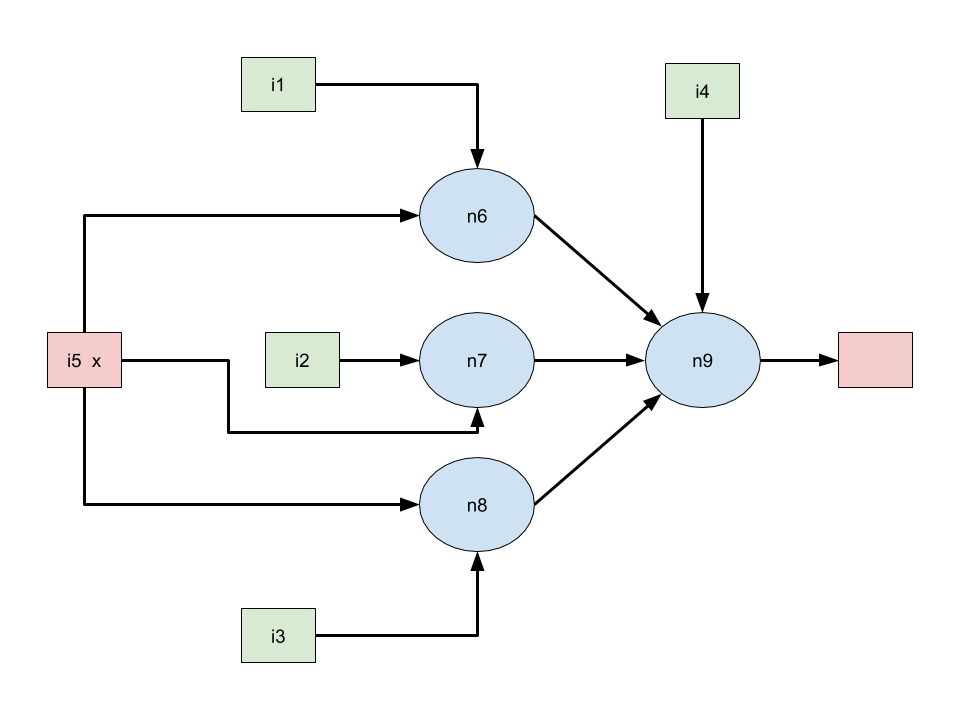
\includegraphics{rede_seno}
  \label{fig:rede_seno}
  \caption{Rede Neural Artificial}
\end{figure}

\section{Função de Treinamento}

A função de treinamento, \texttt{rnaSeno} é apresentada no código a seguir.

\begin{Schunk}
\begin{Sinput}
>   rnaSeno <- function() {
+ 
+   rm(list=ls())
+ 
+   sech2<-function(u)
+   {
+     return(((2/(exp(u)+exp(-u)))*(2/(exp(u)+exp(-u))))) 
+   }
+ 
+   # dados de entrada
+   x_train<-seq(from=0, to=2*pi, by=0.15)
+   x_train<-x_train + (runif(length(x_train))-0.5)/5
+   i <- sample(length(x_train))
+   x_train <- x_train[i]
+ 
+   y_train <- sin(x_train)
+   y_train<-y_train + (runif(length(y_train))-0.5)/5
+ 
+   x_test <-seq(from=0, to=2*pi, by =0.01)
+   y_test <-sin(x_test)
+ 
+   # pesos de entrada
+   i1<-1
+   i2<-1
+   i3<-1
+   i4<-1
+ 
+   w61<-runif(1)-0.5
+   w65<-runif(1)-0.5
+ 
+   w72<-runif(1)-0.5
+   w75<-runif(1)-0.5
+ 
+   w83<-runif(1)-0.5
+   w85<-runif(1)-0.5
+ 
+   w94<-runif(1)-0.5
+   w96<-runif(1)-0.5
+   w97<-runif(1)-0.5
+   w98<-runif(1)-0.5
+ 
+   tol<-0.01
+   nepocas<-0
+   eepoca<-tol+1
+   eta<-0.01
+   maxepocas<-50000
+ 
+   evec<-matrix(nrow=1,ncol=maxepocas) 
+ 
+   while ((nepocas < maxepocas) && (eepoca>tol)){
+     ei2<-0
+     iseq<-sample(length(x_train))
+     for(i in (1:length(x_train))) {
+     
+       i5<-x_train[iseq[i]]
+       y9<-y_train[iseq[i]]
+       
+       u6<-i1*w61+i5*w65
+       i6<-tanh(u6)
+       
+       u7<-i2*w72+i5*w75
+       i7<-tanh(u7)
+       
+       u8<-i3*w83+i5*w85
+       i8<-tanh(u8)
+       
+       u9<-i4*w94+i6*w96+i7*w97+i8*w98
+       i9<-u9
+       
+       e9<-y9-i9
+       
+       d9<-e9
+       
+       dw94<-eta*d9*i4
+       dw96<-eta*d9*i6
+       dw97<-eta*d9*i7
+       dw98<-eta*d9*i8
+ 
+       d6<-sech2(u6)*(d9*w96)
+       d7<-sech2(u7)*(d9*w97)
+       d8<-sech2(u8)*(d9*w98)
+       
+       dw61<-eta*d6*i1
+       dw65<-eta*d6*i5
+ 
+       dw72<-eta*d7*i2
+       dw75<-eta*d7*i5
+ 
+       dw83<-eta*d8*i3
+       dw85<-eta*d8*i5
+ 
+       w61<-w61+dw61
+       w65<-w65+dw65
+ 
+       w72<-w72+dw72
+       w75<-w75+dw75
+ 
+       w83<-w83+dw83
+       w85<-w85+dw85
+ 
+       w94<-w94+dw94
+       w96<-w96+dw96
+       w97<-w97+dw97
+       w98<-w98+dw98
+ 
+       ei<-e9*e9
+       ei2<-ei2+ei
+     }
+     
+     nepocas<-nepocas+1 
+     evec[nepocas]<-ei2
+     eepoca<-evec[nepocas]
+   }
+ 
+   x_calc<-x_test
+   y_calc<-y_test
+ 
+   for(i in (1:length(x_test))) {
+     i5<-x_test[i]
+ 
+     u6<-i1*w61+i5*w65
+     i6<-tanh(u6)
+ 
+     u7<-i2*w72+i5*w75
+     i7<-tanh(u7)
+ 
+     u8<-i3*w83+i5*w85
+     i8<-tanh(u8)
+ 
+     u9<-i4*w94+i6*w96+i7*w97+i8*w98
+     i9<-u9
+ 
+     y_calc[i]<-i9
+ 
+   }
+ 
+   n_test<-length(x_test)
+   erro<-0
+   for(i in 1:n_test)
+     erro<-erro + (y_test[i]-y_calc[i])^2
+ 
+   erro<-erro/n_test
+   erro  
+ 
+   retlist<-list(erro, nepocas, evec[(1:nepocas)], x_test, y_test, y_calc)
+ 
+   return (retlist)
+ 
+ }
\end{Sinput}
\end{Schunk}

\section{Erro médio}

O código a seguir calcula o erro médio, \texttt{mean}, e o desvio padrão \texttt{sd}, para cinco execuções:

\begin{Schunk}
\begin{Sinput}
>   exec1<-rnaSeno()
>   exec2<-rnaSeno()
>   exec3<-rnaSeno()
>   exec4<-rnaSeno()
>   exec5<-rnaSeno()
>   erro<-seq(1:5)
>   erro[1]<-exec1[[1]]
>   erro[2]<-exec2[[1]]
>   erro[3]<-exec3[[1]]
>   erro[4]<-exec4[[1]]
>   erro[5]<-exec5[[1]]
>   mean(erro)
\end{Sinput}
\begin{Soutput}
[1] 0.002038615
\end{Soutput}
\begin{Sinput}
>   sd(erro)
\end{Sinput}
\begin{Soutput}
[1] 0.003369079
\end{Soutput}
\end{Schunk}

\section{Função de saída}

O código a seguir plota o resultado esperado e o resultado da função aproximada:

\begin{Schunk}
\begin{Sinput}
>   exec<-rnaSeno() 
>   x_test<-exec[[4]]
>   y_test<-exec[[5]]
>   y_calc<-exec[[6]]
>   plot(x_test, y_test, type='l', ylim=c(-1,1), col='blue', xlab='', ylab='')
>   par(new=T)
>   plot(x_test, y_calc, type='l', ylim=c(-1,1), col='red', xlab='x', ylab='y')
>   legend(x=4, y=1, legend = c('test','calc'), col = c('blue','red'),pch=c('_','_'))
\end{Sinput}
\end{Schunk}
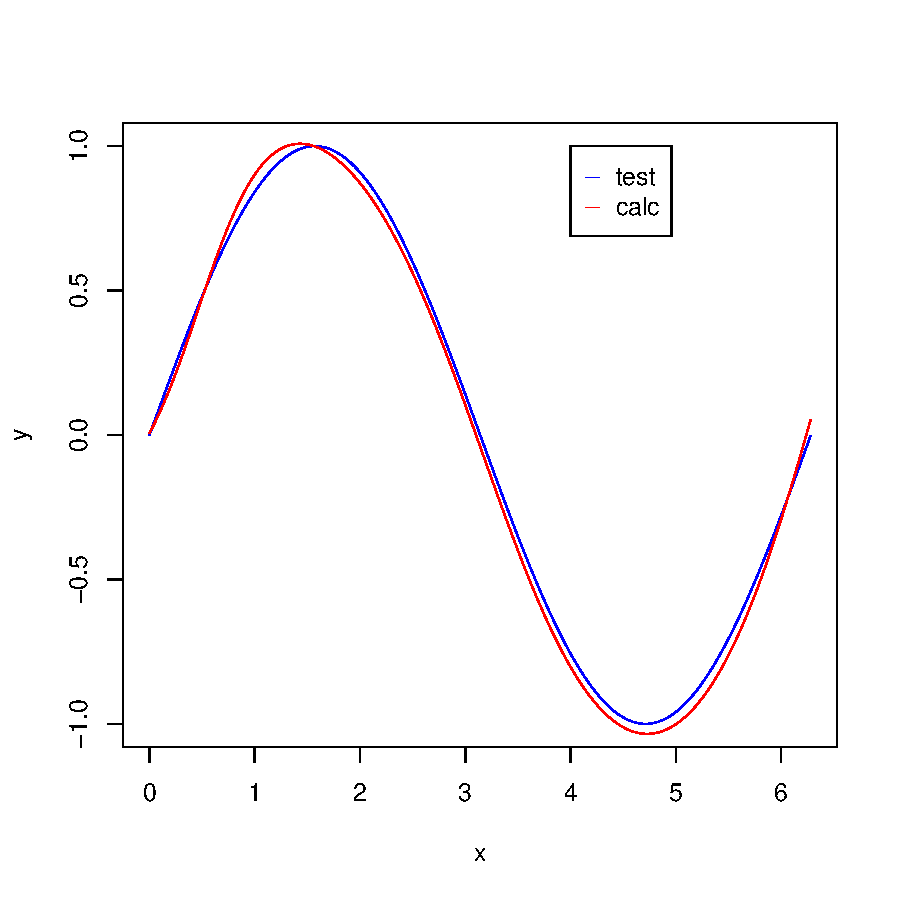
\includegraphics{backpropagation-003}

\end{document}
